\chapter{Modelling integer multiplication as a convolution problem}
\label{chapter:integer_multiplication_convolution}

We now aim to show how the problem of integer multiplication can be phrased as
a convolution problem, and then present a basic algorithm to perform integer
multiplications using the FFT.

Consider $x, y$ two $n$-digit numbers in some base $B$, where $x_0, y_0$ is the
least significant digit.

\section{Integer multiplication as a convolution operation}

Let $\otimes$ be an integer multiplication with delayed carry operation. That
is $u = x \otimes y$ is defined as follows:

\begin{align*}
		u_i & = \sum_{j + k = i} x_j y_k
\end{align*}

Observe how by this definition the operation $u = x \otimes y$ is exactly the
acyclic convolution $u = x \times_A y$. This is further illustrated in figure
\ref{fig:multiplication_convolution}.

\begin{figure}
		\centering
		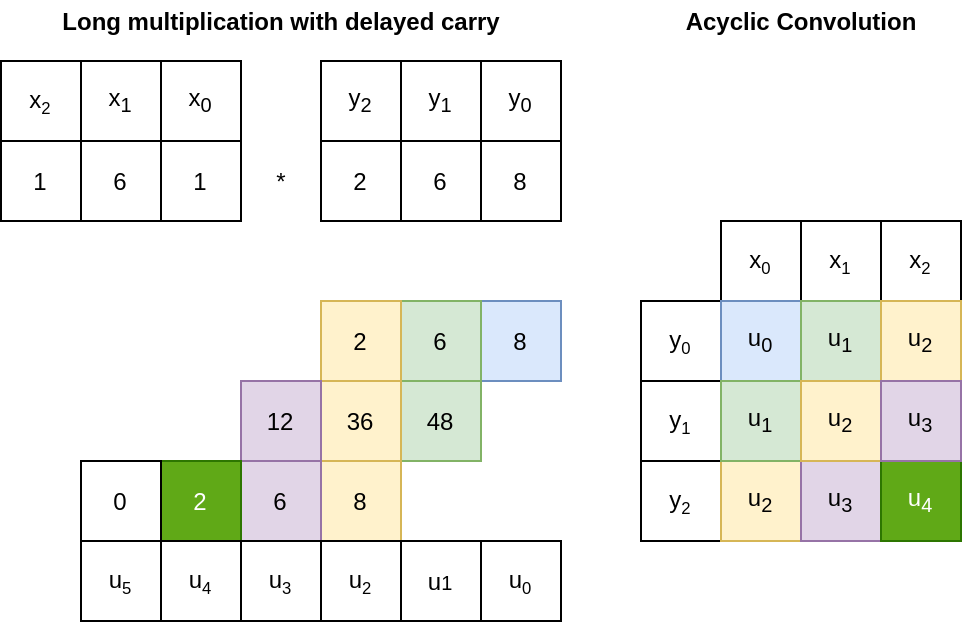
\includegraphics[width=0.6\textwidth]{../resources/multiplication_convolution.drawio.png}
		\caption{Integer multiplication with delayed carry operation is equivalent to acyclic convolution}
		\label{fig:multiplication_convolution}
\end{figure}

\subsection{Applying the delayed carry operation}

Given $u = x \otimes y$, one can calculate the result of a regular
multiplication $v = x \cdot y$ by applying the carry operation. Let
$\intdiv$ denote integer division:

\begin{align*}
		\overline{v}_i & = u_i + (\overline{v}_{i-1} \intdiv B) \\
		v_i & = \overline{v}_i \bmod B
\end{align*}

\section{Integer multiplication with the FFT}

This now allows specification of a basic algorithm for fast integer
multiplication using the FFT, as done by e.g. Crandall and Pomerance, shown in
algorithm \ref{alg:fft_int_mult}.

The algorithm starts by zero-padding the two input signals to length $2n$, and
then calculates $\dft^{-1}(\dft(x_{\text{padded}}) \cdot
\dft(y_{\text{padded}}))$.  Recall that as per sections
\ref{sec:relations_between_convolutions} and \ref{sec:convolution_theorem} this
will thus --- after the rounding required as this generic FFT operates over the
field of complex numbers --- yield the acyclic convolution $x \times_A y$.

The algorithm will then perform the carry operation outlined above, returning
the result $z = x \cdot y$.

\begin{algorithm}
		\caption{Fast integer multiplication with FFT}
		\begin{algorithmic}[1]
				\Function{FFTMult}{$x, y$}
				\State $x \gets$ \Call{Pad}{x, 2n} \Comment{Zero-pad to length $2n$ on high-order side}
				\State $y \gets$ \Call{Pad}{y, 2n}
				\\
				\State $X \gets$ \Call{DFT}{x}
				\State $Y \gets$ \Call{DFT}{y}
				\State $Z \gets X \cdot Y$ \Comment{Dyadic product}
				\State $z \gets$ $\Call{DFT}{Z}^{-1}$
				\State $z \gets$ \Call{round}{z}
				\\
				\State $carry \gets 0$
				\For{$i \gets 0$ to $2n$}
				\State $v \gets z_i + carry$
				\State $z_n \gets v \bmod B$
				\State $carry \gets v \intdiv B$
				\EndFor
				\State \textbf{Return} $z_0 || z_1 || \ldots || z_n || carry$
				\\
				\EndFunction
		\end{algorithmic}
		\label{alg:fft_int_mult}
\end{algorithm}
